\documentclass[a4paper,11pt]{report}
\pdfoutput=1

\usepackage[english,swedish]{babel}
\usepackage[T1]{fontenc}
\usepackage[utf8x]{inputenc}
\usepackage{listings, babel}
\usepackage{graphicx}
\usepackage[colorlinks=true,linktoc=page]{hyperref}
\usepackage[nonumberlist]{glossaries}
\usepackage{subcaption}
\lstset{breaklines=true,basicstyle=\ttfamily}
\usepackage[margin=2cm]{geometry}
\usepackage{lipsum}

\selectlanguage{english}


\newcommand{\image}[4]{
  \begin{figure}[here]
  \centering
  \includegraphics[width=10cm]{images/#1} 
  \caption[#3]{#4}
  \label{fig:#2}
  \end{figure}
}


\title{Fault detection in photovoltaic systems}
\author{David Nilsson, davnils@kth.se}

\newglossaryentry{MPP}
{
  name=MPP,
  description={maximum power point corresponding to an optimal load}
}

\newglossaryentry{MPPT}
{
  name=MPPT,
  description={maximum power point tracking}
}

\newglossaryentry{solar-module}
{
  name=solar module,
  description={An enclosed box containing several interconnected solar cells}
}

\newglossaryentry{iv-curve}
{
  name=I-V curve,
  description={Plot of panel current as a function of panel voltage}
}


\makeglossaries
\glsaddall

\begin{document}
\pagenumbering{gobble}
\maketitle
\newenvironment{abstractpage}
  {\cleardoublepage\vspace*{\fill}\thispagestyle{empty}}
  {\vfill\cleardoublepage}
\newenvironment{polyAbstract}[1]
  {\bigskip\selectlanguage{#1}%
   \begin{center}\bfseries\abstractname\end{center}}
  {\par\bigskip}

\begin{abstractpage}
\begin{polyAbstract}{english}
This master's thesis concerns three different areas in the field of fault detection in PV systems.
Previous studies have concerned homogeneous systems with a large set of parameters being observed, while this study is focused on a more restrictive case.
The first problem is to discover immediate faults occuring in solar panels.
A new online algorithm is developed based on similarity measures within a single installation.
It performs reliably and is able to detect all significant faults over a certain threshold.
The second problem concerns measuring degradation over time.
A modifed approach is taken based on repetitive conditions, and performs well given certain assumptions.
Finally the third problem is to differentiate solar panel faults from partial shading.
Here a clustering algorithm DBSCAN is applied on data in order to locate clusters of faults in the solar plane, demonstrating good performance in certain situations.

\end{polyAbstract}

\begin{polyAbstract}{swedish}
Det här är en uppsats på master-nivå inom fältet feldetektering av fotovoltaiska system.
Tidigare studier har fokuserat på homogena system med en större mängd observerade parametrar, vilket generaliseras i den här studien.
Den första delen är feldetektering av snabba felförlopp i solpaneler.
En ny algoritm presenteras baserad på grader av likhet inom en enskild solpanelsinstallation.
Den presterar väl och är kapabel att hitta alla singifikanta fel över en viss nivå.
Den andra delen består av att mäta degradering av solpaneler över tid.
En variant av tidigare resultat presenteras som baseras på upprepande förhållanden, vilket presterar väl givet vissa antaganden.
Slutligen hanteras detektering av partiell skuggning och urskiljning av detta från riktiga panelfel.
Lösning är en algoritm DBSCAN som hittar kluster av data i solplanet och den påvisar god prestanda i vissa situationer.

\end{polyAbstract}
\end{abstractpage}

\selectlanguage{english}


\tableofcontents

\chapter*{Preface}
\addcontentsline{toc}{chapter}{Preface}
\lipsum[1]

\printglossaries
\cleardoublepage
\addcontentsline{toc}{chapter}{\listfigurename}
\listoffigures
\clearpage
\pagenumbering{arabic}

\chapter{Introduction}
This chapter introduces the purpose of this thesis and gives a general outline of photovoltaic systems and failure detection.
The scope and constraints are described and put into the context of the field of PV (photovoltaic) power electronics, i.e. power generation based on the sun as the energy source.

\section{Photovoltaic power generation}
Power generation based on photovoltaic sources has gradually become an increasingly larger source of power generation during the last few decades~\cite{Zhao2010thesis}.
This trend has been matched with research into more efficient solar panels.
Efficiency is measured as the ratio of incoming sun energy to the maximum attainable output power, with the current record being an efficiency of $44.7\%$~\cite{Fraunhofer2013}.
In addition to research into solar panels there is also an established interest in the surrounding equipment.

Part of these systems are power inverters converting dc energy from the solar panels to the ac grid output.
The efficiency concerns of solar panels naturally extend throughout the system, since any losses will affect the final efficiency of the complete system.
Recently the area of PV inverters has progressed to distributed systems of inverters where a small inverter module is connected to every panel~\cite{Roman2006}.
This is beneficial since each panel can be optimized locally, thereby increasing the energy harvest.
In addition to increased efficiency this also allows individual measurements of solar panels.

These new capabilities provide new possibilities in monitoring of the health of solar panels.
This process, known as fault detection, is an active research area.
Fault detection aims to detect faulty and degraded solar panels as soon as possible. 
Degradation occurs naturally in solar panels and it is of interest to quantify the degradation rate over time.

\section{Purpose of this thesis}
The purpose of this thesis is to study and develop new methods for fault detection in the context of distributed inverter systems.

\subsection*{Problem statement}
Can potential faults in a solar panel, in the context of installations with the specified properties, be detected by studying the available measurements?
This includes the capability of differentiating panel faults from partial shading of the panel.
The problem is how to perform detection efficiently in the presence of different system configurations, but also geographic and thermal dependencies, since all systems deliver different power curves.

\subsection*{Constraints}
The most important scope limitation is that systems should only be studied passively, i.e. the available measurements are used to detect faulty panels.  
Some technical constraints are present as well:
\begin{itemize}
\item The solar panels have 60 or 72 cells built of mono- or poly-crystalline silicon
\item The installations have 14 to 24 panels connected within a small geographic area
\item The available measurements (from each panel) are:
$U$ \footnote{Panel voltage at an optimal load},
$I$ \footnote{Panel current at an optimal load} and
$T_{module}$ \footnote{Low resolution temperature measurement from within the PV inverter}.

\end{itemize}

This reflects the consumer market of smaller panel installations with some of the most common panel types.
The type of solar panels constrains the possible output power range and defines appropriate parameters for testing.
Due to time constraints, the simulation of solar panels has been largely based on existing data streams.
These are used as a basis of generating approximate individual panel curves, limiting the amount of effort required.

The supervising company provides data feeds providing real time measurements of several PV installations in Sweden.
This data is accumulated in a central database for further analysis.
This data has been used in order to verify real-life performance of the classification system, primarily to verify that working systems are not classified as faulty.

Additionally there are other sources that can be used to build realistic simulation models, such as measured solar energy over several years.

\section{Intended readers}
The main target audience interested in this thesis are companies building products in the field of PV power electronics.
Fault detection in solar panels is an active research area and evolves continually, demonstrating an academic interest as well.
The main party interested in the results is of course the supervising company, whom are likely to
integrate a functional solution into their final product.
While being a fairly specialized thesis, it is comprehensible to anyone with a basic background in statistics.
Some basic knowledge of physics and electronic circuits is needed as well in order to fully understand the electrical models.

\section{Sustainability considerations}
From a societal perspective this thesis has mainly a positive impact in three different ways.

The first main improvement is increased efficiency due to faulty solar panels being replaced sooner.
This improvement has a direct benefit in total produced power.
Studies have shown there is a significant power loss due to faults in solar panels.
For example a study conducted in Britain concluded losses upwards $18.9\%$ during the first year of operation~\cite{Firth2010}.
Even though such losses would not be completely eliminated, it is reasonable to conclude that more efficient and reliable detection routines results in faster replacement of faulty panels.

Secondly, early detection of faulty panels results in fewer faulty panels being present in installations.
This implies a reduction in risk of fire hazards~\cite{Zhao2010night} which may affect both personnel and installed equipment.

Thirdly, there is a reduction in labor required for the equivalent amount of monitoring.
The final product should send alerts upon recognizing faulty panels, bypassing any manual supervision of the systems.
In the long term this implies more cost-effective installations and improved sustainability for photovoltaic systems.

\chapter{Background}
This chapter introduces the concept of solar cells, including the underlying physics,
and how they work together with power inverters on the system level.
It is important to have an understanding of the underlying concepts when discussing the applicability of different methods to failure detection.
These concepts are however generic and common knowledge in the field of PV power generation, 
hence this chapter can be skipped given a sufficient existing background.

\section{Theory of the solar cell}
Solar cell technology can be broadly described as equipment converting incoming photons (typically sunlight) to electric energy.
The solar cells of interest in this study are mono- and poly-crystalline silicon, technologies that currently have a large market share~\cite{Zhao2010thesis}.

Both of these share the property of being being constructed around a single pn-junction, i.e. the connection between two differently doped silicon areas.
The incoming photons may be absorbed by the silicon in which case a electron-hole pair is created~\cite{Zhao2010thesis}, since the electron is pushed to an outer layer by the absorbed energy.
Connecting an electric load, such as a heating element, to the terminals of the solar cell will then induce a direct current.
Overall this results in an efficiency of $13-18\%$ for single-junction silicon technology~\cite{Zhao2010thesis}.

The solar cell can by analyzed using an equivalent electrical circuit model with well-defined parameters.
A broadly used model is the one-diode model~\cite{Walker2001} as shown in figure \ref{fig:solar-cell-equiv}.
It is based on modelling the solar cell as a current source connected in parallel with a diode.
In addition there are inherent losses due to imperfect manufacturing.
These are modelled as a series and a parallel resistance.
The resulting current $I_{load}$ flows across the terminals through a load with potential difference (voltage) $U_{load}$.
$I_{photo}$ corresponds to the amount of current generated by incoming photons which is proportional to the irradiance and area of the solar cell.

\begin{figure}[!ht]
\centering
\begin{subfigure}{0.4\textwidth}
  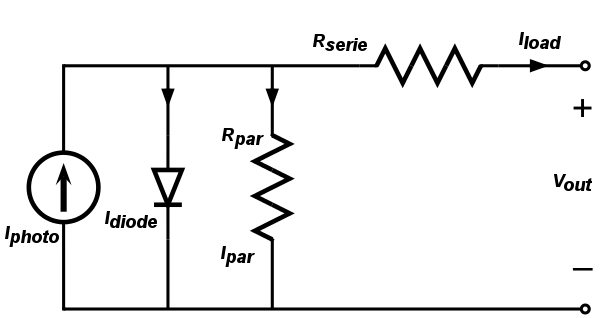
\includegraphics[width=\linewidth]{solar-cell-equiv.png}
\end{subfigure}
~
\begin{subfigure}{0.4\textwidth}
  \begin{tabular}[b]{| c | c |}
  \hline
  $I_{load}$ & load current \\ \hline
  $U_{load}$ & load voltage\\ \hline
  $I_{photo}$ & photogenerated current \\ \hline
  $I_{diode}$ & diode current \\ \hline
  $I_{par}$ & parallel loss current \\ \hline
  $R_{par}$ & parallel loss resistance \\ \hline
  $R_{serie}$ & series loss resistance \\ \hline
  \end{tabular}
\end{subfigure}
  \caption[Equivalent circuit of a solar cell]{
    \emph{
    Equivalent circuit of a solar cell based on a current source and diode,
    with losses represented by a series and a parallel resistance.
    The table describes all variables of the one-diode model.
    }
  }
  \label{fig:solar-cell-equiv}
\end{figure}

\clearpage
The model can be formalized in order to solve for the resulting current and voltage, given the parameters of a solar cell.
Summing up all the currents it holds that $I_{photo} = I_{diode} + I_{par} + I_{load}$.
Using the well known Ohm's law followed by Shockley's diode equation~\cite{Walker2001}, the following holds:

\begin{multline}
\label{eq:eq-circuit}
I_{load} = \\
I_{photo} - I_{diode} - I_{par} = \\
I_{photo} - I_{diode} - \frac{R_{serie}I_{load} + U_{load}}{R_{par}} = \\
I_{photo} - I_{sat}(e^\frac{q(R_{serie}I_{load} + U_{load})}{k_B T} - 1) - \frac{R_{serie}I_{load} + U_{load}}{R_{par}}
\end{multline}

$I_{sat}$ denotes the constant saturation current of the diode,
$k_B \approx \SI{1.38e-23}{\joule\per\kelvin}$,
and $q \approx \SI{1.60e-19}{\coulomb}$.

The free variables are $I_{load}$, $U_{load}$ and $T$, where $T$ is the temperature measured at the p-n junction.
All parameters of the model, such as $I_{sat}$, may be given in a datasheet or can alternatively be extracted by performing non-linear regression based on samples of the free variables~\cite{Walker2001}.

There are several relevant aspects in understanding this equivalent model when performing analysis of power generated from solar panels.
Firstly the output current is proportional to the incoming irradiance, which directly affects $I_{photo}$.
Figure $\ref{fig:trina-iv-curve}$ shows a plot of $I_{load}$ as a function of $U_{load}$ at different irradiations.
The panel is held at a constant temperature.

\image{trina-60cell-iv-alpha.png}{trina-iv-curve}{Solar panel IV-curve characteristic}{
  Typical IV-curve of a solar panel. Note the non-linear relationship between voltage and current, and the effect of solar irradiation on output current.
}

In addition to changing irradiation there might also be a range of operating temperatures depending on local weather conditions.
The temperature affects the second term in equation \ref{eq:eq-circuit} and increased temperature results in decreased load current.
This is important to take into account since otherwise increased temperature might be mistaken for decreased irradiation.
While being an important source of measurements in general, this study only concerns fault detection based on samples of $I_{load}$ and $U_{load}$, but still needs to perform reliable classification.

Finally, it is important to realise that different solar panels have different parameters and will yield different I-V curves.
This implies that inhomogeneous systems offer challenges when comparing produced power output, for example in the case of fault detection.

\section{Systems of solar panels}
Single solar cells of the types described previously typically generate an output voltage of \SIrange{0.6}{0.7}{\volt}~\cite{Zhao2010thesis}.
A solar module connects several solar cells and places them into a rigid enclosure.
This module can then be mounted as part of a larger system.
Figure \ref{fig:solar-module-generic} shows a 54-cell module with the output dc terminals visible on the backside.

\image{solar-module-generic.jpg}{solar-module-generic}{Generic solar module}{
  Back and front of a generic 54-cell silicon solar module. Every cell and the vertical interconnections are clearly visible.
}

In addition to protecting the fragile silicon sheets, the purpose of the module is also to improve yield by using an anti-reflective coating.
This thesis considers modules containing 60 or 72 solar cells of the previously specified type, connected in series.
The resulting I-V curve of the module has an increased width and every point is stretched to $n \cdot U_{load}$ with $n$ cells each producing at some $U_{load}$.

There is however also some extra components involved in the module circuitry.
The panel is divided into y substrings of which each has a diode connected in parallel.
During normal operation the diodes will not carry any current.
If some cell is reduced in performance, for example by having an unusually high series resistance, this will result in the corresponding diode conducting the current, effectively bypassing that specific substring~\cite{Roman2006}.
This is relevant since the I-V curve will reflect these properties and should be analyzed while keeping these effects in mind.

\section{The role of PV inverters}
Solar panels produce direct current as previously described.
This is suitable for certain types of applications such as charging batteries.
It is however not suitable for generation on the electric grid which uses ac power at a fixed voltage.
This conversion is done using a power inverter, also known as PV inverter.
There are different topologies applicable, i.e. different arrangements of both solar panels and PV inverters.
Traditionally a common configuration has been to use long strings of modules connected in series with a single big inverter at the end of the string.
This approach is however constrained due to individual modules having an unproportional influence on the total power yield of the string~\cite{Roman2006}.

\image{optistring-inverter.jpg}{optistring-inverter}{Optistring PV inverter}{
  The distributed Optistring PV inverter with dc input and ac output.
  A separate inverter is placed on the back of every solar panel.
}

The system considered in this study is a distributed version with a typical inverter shown in figure \ref{fig:optistring-inverter}.
Each module has its own simple PV inverter acting as an independent ac power source.
In addition to providing higher efficiency, this also produces $I_{load}$ and $U_{load}$ measurements from every individual module.
This is highly relevant since studies in fault detection typically consider a specific topology and the results might not always generalize to the distributed case.

A PV inverter should transform the power in the most efficient way and more specifically ensure that the panel is being applied to an optimal load.
This corresponds to finding the point on the I-V curve where $I_{load} \cdot U_{load}$ is maximal.
This maximum power point (MPP) is typically found using methods that search along the I-V curve.
Examples include Pertube and Observe and Incremental Conductance~\cite{Roman2006}.
These are relevant to this study since local searches may not be well-behaved during panel faults~\cite{Roman2006}.
This is due to the existence of multiple local maxima on the I-V curve, resulting in the possibility of considering a local optima as a global maxima.
Previous studies have also found that MPP tracking (MPPT) might prevent faults from being observed during night-to-day transitions~\cite{Zhao2010night}.

A relevant term applicable to measuring the efficiency of solar cells is \emph{fill factor} which is defined as the ratio between the power at $I_{MPP} \cdot U_{MPP}$ and $I_{max} \cdot U_{max}$.
The maximum reference values are defined as $I_{max}$ being the current measured in closed circuit and $U_{max}$ being the voltage measured without any load connected.


\section{Solar power in practice}
Given an understanding of the different components of a PV solar installation it is also important to reflect on real-life behaviour.
The power output of an installation and individual solar panels vary to a large degree.
Figure \ref{fig:january-power-curve} and \ref{fig:october-power-curve} illustrate this, where a 10-fold decrease in peak power output is seen over a period of 3 months.
In addition the total duration of power output is reduced by 4 hours.
Another interesting aspect of these graphs is the significant amount of noise present due to shadowing.

\begin{figure}[here]
\centering
\subimage{january-power-curve.png}{january-power-curve}{TBD}{
   Power curve captured during a day in January 2014.
}{0.48}
~
\subimage{october-power-curve.png}{october-power-curve}{TBD}{
  Power curve captured during in a day in October 2013. Note the use of a different scale on the Y-axis.
}{0.48}
\caption[Power curves captured from an installation]{\emph{Power curves (in Watt) captured from a 16-module installation based in Stockholm, Sweden.}}
\end{figure}

After sunset and during periods of negligible irradiance the system is completely shutdown.
This is done in order to reduce power consumption and thereby increase overall efficiency.
In addition to seasonal and geographical dependencies, the power output is also proportional to the number of solar panels in the system and the type of each panel.
All of these highly varying conditions impose restrictions on how fault detection can be implemented and the required scope of validation.
The main point is that developed methods need to be dynamic and adaptive to any applicable system configuration.

\chapter{Theory of fault detection}
Based on knowledge of how a PV system produces energy and the underlying dependencies,
it is possible to reason about faults.
Faults in PV systems can be characterized as permanent power losses but a more fine-grained analysis might be suitable if there are failure-specific patterns that can be utilized.
This chapter gives an overview of possible failure conditions and describes the different kinds of methods that have been established by previous studies.

\section{Issues in photovoltaic systems}
There are a lot of studies analyzing different issues present in PV systems \cite{Baltus1997,King2002,Petrone2008}, demonstrating an interest in detecting faults to the greatest extent as early as possible.

A study conducted in Spain~\cite{Munoz2011} discusses the following failures in solar modules:
\begin{itemize}
\item Yellowing and browning
\item Delamination
\item Bubbles in the solar module
\item Cracks in cells
\item Defects in anti-reflective coating
\item Hot spots caused by the panel acting as a load
\end{itemize}

Another study~\cite{Forman1982} identified the following conditions:
\begin{itemize}
\item Edge-seal delamination
\item Newly cracked cells
\item Delamination over cells and interconnections
\item Split encapsulation over cells and interconnections
\item Protruding interconnections
\end{itemize}

It has also been found that connections and the welds can degrade over time \cite{Houssein2010}.

In conclusion it can be said that there is a wide range of failure conditions.
This breadth motivates the use of classes of failures, based on the electrical properties induced during a fault.
\cite{Zhao2010thesis} and the papers \cite{Zhao2012tree,Zhao2013graph,Zhao2013outlier} use a categorization into ground faults, line-line faults, and open-circuit faults.
Ground faults are defined as a conductor accidentally having contact with the system ground~\cite{Zhao2010thesis}.
Line-line faults occur when two different potentials conduct by accident~\cite{Zhao2010thesis}.
Open-circuit faults occur when a conductor is accidentally removed from a closed circuit~\cite{Zhao2010thesis}.
The same study concludes that ground and line-line faults typically exhibit a significant drop in output voltage,
but also states that open-circuit faults and degradation causes significant decrease in current.

The same thesis found that protection devices commonly present in PV installations known as over-current protection devices (OCPD) and ground protection (GPD) are not sufficient.
During certain kinds of faults the MPPT may interfere and lower the current output, which in turn will not trigger the current-based protection devices.
Similar issues are present when faults occur during the night \cite{Zhao2010night}.

In the context of degradation over time it has been found that dust is a significant problem \cite{Mani2010}.
These effects are however very dependent on the geographical position and the physical alignment with respect to weather conditions.

A study \cite{Munoz2011} found that early degradation occurs due to wide variety for reasons.
The paper ties the measured degradation rates to a specific allowance, based on guarantees from the manufacturer.
It discusses a typical guarantee of $90\%$ over 10-15 years and $80\%$ over 20-25 years in preserved nominal power.

Meyer and Dyk~\cite{Meyer2004} note that degradation in the anti-reflective coating results in a brightening in the color of the cell.
It can also be detected in the module's maximum attainable voltage and current.
The paper discusses solar cell degradation as three different factors being involved in relation to the one-diode model figure \ref{fig:solar-cell-equiv}.
The first is an increase in series resistance, the second is a decrease in the parallel resistance (which implies a larger loss current), and the third being deterioration of the anti-reflection coating affecting the photogenerated current.

Concrete percentual figures of degradation have also been studied~\cite{Quintana2002}, which cites a degradation rate of about $0.7\%$ per year for multi-crystalline modules.
There is also a note on that the system may continue to operate in degraded conditions without causing an intermediate failure.
The paper also describes a condition known as \emph{light induced degradation} (LID) which is a module degradation
that occurs during the first few hours of sunlight exposure.
It is stated that at most a $5\%$ degradation in maximum attainable current has been observed.

\section{Partial shading of solar panels}
Partial shading occurs when a subset of the PV array is shaded to some degree.
This occurs naturally for example due to passing clouds.
Nearby obstacles might also interfere and cast shadows, resulting in reduced power output.
Hence shading conditions is a relevant aspect when planning a PV installation.
Due to the nature of the resulting power reduction it is also relevant to classify power output into either the case of partial shading or faulty panels.

Some studies, e.g. \cite{Stettler2005}, view partial shading as another failure condition.
This somewhat simpler view does not require partial shading to be separated from for example faulty solar panels.

Partial shading has been studied in isolation \cite{Alsayid2013}.
The paper illustrates the effect of bypass diodes triggered due to shadow conditions, resulting in non-smooth IV-curves with different characteristics.
However, it does not describe suitable classification attributes or relate shading to fault conditions.
The results are also heavily dependent on the panel topology and placement of bypass diodes.

A study based on measurements in the UK \cite{Firth2010} considers classification of faults as partial shading.
The approach taken is to, based on the position of the sun, measure the frequency of errors at individual segments in the solar plane.
The solar plane is viewed as solar elevation on the y axis and solar azimuth on the x axis.
Small 5-minute segments of this plane are then considered in isolation.
A fault is considered as partial shading if the frequency of faults in the corresponding segment is higher than an experimentally calculated threshold.
The actual frequency is simply calculated as the number of failure-free occurrences of the segment with respect to the number of faults within the segment.

\clearpage
\section{Approaches to fault detection}
A basic approach to detecting unexpected power loss is comparing the output with a reference value and triggering an alarm when large differences are detected.
The approach taken in~\cite{Stettler2005} is to perform monitoring using satellites, essentially building up known weather conditions.
This approach is not applicable to this study due to insufficient weather data available.

An extension to this method is building an analytical model \cite{Chouder2010,Raina2013,Chao2008}
based on the one-diode model introduced previously (equation \ref{eq:eq-circuit}).
All parameters are retrieved from the manufacturers datasheet or through parameter extraction \cite{Eicker2005,Chouder2009,Walker2001}.
This method relies on access to both irradiance and solar panel temperature measurements in order to calculate the reference MPP.
This is then compared to the measured working point as previously discussed.

An active approach is described in \cite{Meyer2004}, where the whole IV-curve is studied for defects, and the maximum attainable $U_{max}$ and $I_{max}$ are recorded over time.
Due to the nature of sweeping IV-curves this implies that this gives a reduction in power output during the analysis.
In addition it is not applicable to passive studies of systems since they can be assumed to deliver output at MPP.

Two studies by Vergura et al.~\cite{Vergura2008,Vergura2009} consider several identical PV string and compares the outputs in order to classify significant deviations.
This is done by checking if certain statistical assumptions can be made, formally that the power differences are independently normally distributed with identical variance.
If this is the case a method known as analysis of variance (ANOVA)~\cite{Vergura2009} can be applied in order to build confidence interval for the power output of each PV string.
Otherwise the Kurskal-Wallis test~\cite{Vergura2009} is applied in order to build the corresponding intervals.
The resulting confidence intervals can be studied for significant deviations which would imply defect solar modules.
While not being directly applicable to this study, the papers remain relevant due to the basic assumption of only having access to power measurements.

Another statistical approach is taken by Zhao~\cite{Zhao2013outlier} that is centered around outlier detection.
Similarly to \cite{Vergura2008,Vergura2009}, the Zhao paper assumes a set of identical PV strings and tries to classify deviations.
This is done by building confidence intervals using three different methods: 3-Sigma rule, Hampel identifier, and Boxplot rule.
All of the surveyed methods exhibit different properties but the paper concludes that the Hampel identifier and Boxplot rule are suitable for fault detection.
Based on the assumptions made, the paper can consider all PV string currents as samples taken from a single normal distribution, allowing straight-forward statistical analysis.
This simplification is however not directly applicable to this study.

In the case of given knowledge surrounding faults it is possible to apply supervised learning, e.g. \cite{Zhao2012tree},
where a labelled dataset is available containing measurements classified manually.
This dataset can for example be generated by measuring voltage and current of solar modules while injecting faults.
The paper discusses a decision tree model that takes the available measurements and locates the most probable classification based on the dataset.
Classification performance is concluded to be very good but real-life applications are limited due to the dataset being heavily tied to a specific PV installation.

A natural extension is analyzed in \cite{Zhao2013graph} which considers the case of graph-based semi-supervised learning, where only a small amount of reference data is available from the start.
This approach results in significant cost reductions, due to the low amount of labeled data, but is also possible to adapt to changing conditions in different systems.
The classification performance is up to $99\%$ for certain classes of errors.

Finally, \cite{Kang2012} takes the approach of using a Kalman filter in order to predict power output.
The Kalman filter~\cite{Kang2012} takes a set of noisy measurements and the underlying physical model, and produces the most probable output value in an iterative process.
This is used in order to locate faults based on measurements of voltage, current, and panel temperature.
Notably this permits classification without access to irradiance data.
The requirement of access to to panel temperature is however limiting in the context of this report.

There has also been research into locating the faulty panel within a string~\cite{Lin2012}.
These results can be considered less applicable when individual solar module measurements are available.

\section{Measuring degradation}
Panel degradation needs to be measured in order to quantify the losses due to possible faulty panels that may void any established guarantee conditions.
Traditionally several different manual techniques have been utilized~\cite{Munoz2011} such as IR-based camera snapshots, exposure to strong light, and I–V curve analysis string by string.

The PVSAT project~\cite{Stettler2005} considers faults based on their long-term effects.
Losses are classified as panel degradation after a long period of time has passed with an energy reduction in the range of $0-20\%$.

A recent master's thesis~\cite{Zhao2010thesis} simulates degradation in order to test the implemented methods.
In this model a variable series resistance is introduced in the solar module.
The resistance is then gradually increased over time in order to provide a significant decrease.
This loss corresponds to $R_{serie}$ in the one-diode model (figure \ref{fig:solar-cell-equiv}).

One approach to detecting degradation is measuring the fill-factor over time~\cite{Raina2013}.
The fill factor is calculated by approximating the maximum attainable current and voltage through parameter estimation.
The cited study is however constrained to installations with measurements of irradiance and temperature, and hence not applicable to this report.

Finally, \cite{Makrides2010} evaluates degradation over longer time periods by using several techniques.
The study assumes access to irradiation and temperature and samples the produced power during periods of high irradiance.
All measurements are normalized by considering both the irradiance and temperature conditions.
These values are then averaged on a monthly basis using a least squares method.
Annual degradation can then be quantified by comparing months pairwise over a year.
The study makes an important remark regarding changing conditions during individual days, where all considered panel technologies suffered output losses as the day progressed.
This is attributed to changing spectral conditions.

\section{Summary}
%TODO
% {\color{red} This section will draw conclusions regarding the applicability of various methods to this specific study.}
The constraints of thesis also affect the applicability of many of the previously mentioned methods.
Firstly, the constraint of only having access to voltage, current, and low-precision temperature values restricts the immediate applicability of many methods.
The lack of irradiance measurements contributes to a more general setting in the case of the one-diode model, since the $I_{photo}$ value needs to be considered unknown.
Since the temperature is not measured at the PN-junction, the corresponding term in the one-diode model needs to be modelled as an expression of the actual measured value.
In general this contributes to a very general theoretical model which not necessarily can be fitted onto a set of data samples, as described in studies based on an analytical model.

Secondly, it is important to distinguish between the cases of having several identical PV strings or panels, from the case of several panels with possibly different characteristics.
This implies that the methods based on outlier detection do not transfer naturally, since the offsets between panels need be taken into account.

Detection of partial shading does not have the same dependency on specifics on the solar installation, since it only assumes access to an existing flow of fault classifications.
The method of studying a solar plane and correlations with the reported faults is suitable for this thesis.

Degradation measurements are also affected by the lack of irradiation and junction-level temperature measurements.
The studies mentioned rely on correcting for these factors when comparing two points in time, in order to determine the degradation in power output.
Hence another approach would be to generalize this procedure for the case unknown irradiance and a model of the junction-level temperature.

\chapter{Implementation}
This chapter describes the approaches that have been taken to solve the problems stated in the introduction.
Each section is described separately with algorithmic outlines and general comments regarding applicability within the scope of this thesis.

\section{Simulation framework}
A central part of this thesis has been to develop a simulation framework in order to study the different problems in various aspects.
This is necessary since a algorithmic approach to e.g. fault detection needs to be evaluated under real life conditions.
It is also important to take different system characteristics and system configurations into account when presenting classification results.

The simulation framework consists of several parts.
It is implemented as a driver program which interfaces towards a database, either generating data or fetching data for e.g. classification purposes.

Data generation has been implemented based on real life measurements of yearly irradiance and temperature values gathered at a location in Stockholm, Sweden.
These inputs are used together with the parameters of a solar installation, in order to generate a resulting series of voltage, current, and temperature values at 5 minute intervals.

%TODO

The second part of the data generation is injecting faults into output of solar installations.
This has been implemented as a fault occurring at some fixed point in time, with an independent percentage loss in voltage and current.
These faults may also occur during night or during low irradiance conditions, as motivated by the possible classification difficulties previously discussed.

The generated data has then been used in order to determine classification performance.
This has been implemented as some external procedure receiving input measurements from a whole installation over time.
Hence this approach reflects real life use cases where online classification is performed.
Repeating this process over many different systems with different configuration results in statistically significant results, applicable to systems concerned in this thesis.
The procedures being applied on the data streams are described in the following sections.

\section{Immediate failure detection}
%TODO
Discussion on how immediate failure detection was implemented, with some basic code constructs.

Describe implementation of online algorithm.
Discuss choice of threshold parameters.

\section{Measuring degradation}
%TODO
Discussion on how degradation measurement was implemented.

Describe taking the approach of fitting data using one-diode model.
Discuss difficulties relating to amount of data available, computation constraints.
Describe alternative approach based on epsilon-close samples.
Plot the corresponding precision plot.

% build a N(x,y)-like graph over measured degradation in all non-faulty modules
% each error can be seen as a scalar (real - estimate)
% plot the distribution of these.
% might need additional data, but the graph can be extended later (something like ~200 samples should be doable?)
% both graphs basically describe the same property but in different ways

% should voltage and current be presented separetely? this implies 2x2 plots in total. that's reasonable.

\section{Detection of partial shading}
%TODO
Discussion on how partial shading detection was implemented.

Discuss solar plane and auto correlation methods.

% use data sourced from the KTH system, detect faults, and run the clustering algorithm on the results
% choose appropiate parameters as functions of the number of faults.
% the resulting graph should show shading as clusters in the solar plane, possibly the coloured graph, but likely only the outlined version.

\chapter{Results}
%TODO
Result chapter with results such as classification rate and various graphs.

\section{Immediate failure detection}
%TODO
Discussion of how immediate failure detection performs.

\begin{figure}[here]
\centering
\subimage{classification-voltage}{classification-voltage-plot}{TBD}{
   TBD
}{0.48}
~
\subimage{classification-current}{classification-voltage-plot}{TBD}{
  TBD
}{0.48}
\caption[TBD summary]{\emph{TBD description}}
\end{figure}

\section{Measuring degradation}
%TODO
Discussion of how degradation measurements perform.

\subsection{Epsilon method}
\begin{figure}[here]
\centering
\subimage{degrad-voltage-error}{degrad-voltage-error-plot}{TBD}{
   TBD
}{0.48}
~
\subimage{degrad-voltage-ratio}{degrad-voltage-ratio-plot}{TBD}{
  TBD
}{0.48}
\caption[TBD summary]{\emph{TBD description}}
\end{figure}

\begin{figure}[here]
\centering
\subimage{degrad-current-error}{degrad-current-error-plot}{TBD}{
   TBD
}{0.48}
~
\subimage{degrad-current-ratio}{degrad-current-ratio-plot}{TBD}{
  TBD
}{0.48}
\caption[TBD summary]{\emph{TBD description}}
\end{figure}

\section{Detection of partial shading}
%TODO
Discussion of how partial shading classification performs.


\begin{figure}[here]
\centering
\subimage{solar-plane-faults}{solar-plane-faults-plot}{TBD}{
  % parameters used: epsilon 8, min pts 3, eucledian distance R^2
  TBD
}
{0.48}
~
\subimage{kth-panels}{kth-panels-image}{TBD}{
  TBD
}{0.48}
\caption[TBD summary]{\emph{TBD description}}
\end{figure}

\image{solar-plane}{solar-plane-plot}{TBD}{
  TBD
}

\chapter{Conclusions}
%TODO
General conclusions on the results and how they fit into todays industry and state-of-the-art research.
Reflect on each of the three categories separately.
Discussion on simulation vs real-life PV installations.
Discussion on future work.

\bibliographystyle{abbrv}
\bibliography{../ref.bib}

\end{document}
